%-----------------------------------------
% Note: Use pdflatex to process this file.
%
% IMPORTANT: This file uses .aux files from the Bmad and Tao manuals so pdflatex these manuals beforehand.
%            Note: It is assumed that the bmad, tao, and examples directories are all on the same level.
%-----------------------------------------

%\documentclass{article}
\documentclass{hitec}     % Tutorial overall style

\usepackage{index}
\usepackage{xr}
\usepackage{textgreek}
\usepackage{setspace}
\usepackage{graphicx}
\usepackage{moreverb}    % Defines {listing} environment.
\usepackage{amsmath, amsthm, amssymb, amsbsy, mathtools}
\usepackage{alltt}
\usepackage{rotating}
\usepackage{enumitem}
\usepackage{subcaption}
\usepackage{toc-dcs}    % See toc-dcs.sty file in this directory.
\usepackage{xspace}
%%\usepackage{makeidx}
\usepackage[section]{placeins}   % For preventing floats from floating to end of chapter.
\usepackage{longtable}  % For splitting long vertical tables into pieces
\usepackage{multirow}
\usepackage{booktabs}   % For table layouts
\usepackage{yhmath}     % For widehat
\usepackage{xcolor}      % Needed for listings package.
\usepackage{listings}
\usepackage[T1]{fontenc}   % so _, <, and > print correctly in text.
\usepackage[strings]{underscore}    % to use "_" in text
\usepackage[nottoc,numbib]{tocbibind}   % Makes "References" section show in table of contents
\usepackage[pdftex,colorlinks=true,bookmarksnumbered=true]{hyperref}   % Must be last package!

%----------------------------------------------------------------

\newcommand{\Bf}[1]{{\bf #1}}
\newcommand{\dsfrac}[2]{\frac{\displaystyle #1}{\displaystyle #2}}
\newcommand{\calO}{{\cal O}}
\newcommand{\calH}{{\cal H}}
\newcommand{\Cal}[1]{{\cal #1}}
\newcommand{\two}{}
\newcommand{\bfsig}{\boldsymbol{\sigma}}
\newcommand{\bfbeta}{\boldsymbol{\beta}}
\newcommand{\bfphi}{\boldsymbol{\phi}}
\newcommand{\bfeta}{\boldsymbol{\eta}}
\newcommand{\sigb}{\sigma_\beta}
\newcommand{\bfrbar}{\overline{\Bf r}}
\newcommand{\BF}[1]{{\text{\bf #1}}}
%%\newcommand{\BF}[1]{{\normalfont\textbf{#1}}}

\newcommand{\re}{\operatorname{Re}}
\newcommand{\im}{\operatorname{Im}}

\newcommand{\bfa}{\Bf a}
\newcommand{\bfg}{\Bf g}
\newcommand{\bfk}{\Bf k}
\newcommand{\bfq}{\Bf q}
\newcommand{\bfr}{\Bf r}
\newcommand{\bfx}{\Bf x}
\newcommand{\bfz}{\Bf z}
\newcommand{\bfA}{\Bf A}
\newcommand{\bfB}{\Bf B}
\newcommand{\bfC}{\Bf C}
\newcommand{\bfE}{\Bf E}
\newcommand{\bfG}{\Bf G}
\newcommand{\bfH}{\Bf H}
\newcommand{\bfI}{\Bf I}
\newcommand{\bfL}{\Bf L}
\newcommand{\bfM}{\Bf M}
\newcommand{\bfO}{\Bf O}
\newcommand{\bfQ}{\Bf Q}
\newcommand{\bfK}{\Bf K}
\newcommand{\bfP}{\Bf P}
\newcommand{\bfR}{\Bf R}
\newcommand{\bfS}{\Bf S}
\newcommand{\bfV}{\Bf V}
\newcommand{\bfT}{\Bf T}
\newcommand{\bfU}{\Bf U}
\newcommand{\bfW}{\Bf W}

\newcommand{\vdot}[2]{\Bigl[ #1, \, #2 \Bigr]}
\newcommand{\comma}{\> ,}
\newcommand{\period}{\> .}
\newcommand{\bfAbar}{\overline{\bfA}}
\newcommand{\bfCbar}{\overline{\bfC}}
\newcommand{\bfKbar}{\overline{\bfK}}
\newcommand{\bfkbar}{\overline{\bfk}}
\newcommand{\bfTbar}{\overline{\bfT}}
\newcommand{\Hbar}{{\overline{H}}}
\newcommand{\Kbar}{\overline{K}}
\newcommand{\kbar}{\overline{k}}
\newcommand{\Pbar}{\overline{P}}
\newcommand{\gam}{\gamma}                                     
\newcommand{\inv}{^{-1}}

\newcommand{\tot}{{\text{tot}}}

%%\newcommand{\dotproduct}{\mathbin{\scriptscriptstyle\stackrel{\bullet}{{}}}}
\newcommand{\dotproduct}{\mathbin{\boldsymbol{\cdot}}}
\newcommand{\cross}{\mathbin{\boldsymbol{\times}}}

\newcommand{\what}{\widehat}
\newcommand{\wt}{\widetilde}
\newcommand{\bfhat}[1]{{\widehat{\bf  #1}}}
\newcommand{\bftilde}[1]{{\widetilde{\bf #1}}}
\newcommand{\xw}{{\widetilde x}}
\newcommand{\yw}{{\widetilde y}}
\newcommand{\rw}{{\widetilde r}}

\newcommand{\tstyle}{\textstyle}
\newcommand{\stilde}{{\widetilde s}}
\newcommand{\tWl}{\widetilde{W}^{SR}_\parallel}
\newcommand{\WlS}{W^{SR}_\parallel}
\newcommand{\WtS}{W^{SR}_\perp}
\newcommand{\WtL}{W^{LR}_\perp}

\newcommand{\hyperbf}[1]{\textbf{\hyperpage{#1}}}
\newcommand{\Hyperref}[2]{\index[routine]{#2}\hyperref[#1]{#2}}

\newcommand{\om}{\omega}
\newcommand{\qqquad}{\qquad \qquad}
\newcommand{\ks}{\widetilde k_s}
\newcommand{\kone}{\widetilde k_1}

\newcommand{\hphphp}{\hphantom{\dfrac{k_x}{k_y}}}
\newcommand{\Ce}{\text{C}}
\newcommand{\Se}{\text{S}}
\newcommand{\Ch}{\text{Ch}}
\newcommand{\Sh}{\text{Sh}}

\newcommand{\CR}{\\}
\newcommand{\CRNO}{\nonumber \\}
\newcommand{\dstyle}{\displaystyle}

\newcommand{\fig}[1]{Fig.~\ref{#1}}
\newcommand{\figs}[1]{Figs.~\ref{#1}}

\newcommand{\pow}[1]{\cdot 10^{#1}}
\newcommand{\tao}{{\sl Tao}\xspace}
\newcommand{\bmad}{{\sl Bmad}\xspace}
\newcommand{\mad}{{\sl MAD}\xspace}
\newcommand{\quickplot}{{\sl Quick Plot}\xspace}
\newcommand{\cpp}{$C$\hskip-0.3ex\protect\raisebox{0.2ex}{\scriptsize ++}\xspace}
\newcommand{\CPP}{$C$\hskip-0.3ex{\protect\raisebox{.3ex}{\large {+}+}}\xspace}
%%\newcommand{\CPP}{$C${\small ++}\xspace}

\newcommand{\eq}[1]{{(\protect\ref{#1})}}
\newcommand{\Eq}[1]{{Eq.~(\protect\ref{#1})}}
\newcommand{\Eqs}[1]{{Eqs.~(\protect\ref{#1})}}

\newcommand{\svn}{\vn{Subversion}\xspace}
\newcommand{\sref}[1]{\S\ref{#1}}
\newcommand{\Sref}[1]{Sec.~\sref{#1}}
\newcommand{\extref}[1]{\S\ref*{#1}}   % No hyperlink. For external refs. \extref
\newcommand{\cref}[1]{Chapter~\ref{#1}}

\newcommand{\toffset}{\vskip 0.01in}
\newcommand{\rot}[1]{\begin{rotate}{-45}#1\end{rotate}}

\newcommand{\ave}[1]{\left\langle #1 \right\rangle}

\newcommand{\vn}{\begingroup\catcode`\_=11 \catcode`\%=11 \dottcmd}
\newcommand\dottcmd[1]{{\usefont{T1}{lmss}{bx}{n} #1}\endgroup}

%\newcommand\ttverb{
%  \bgroup\let\do\@makeother\dospecials\catcode`{=1 \catcode`}=2 \DSAcode}
%\newcommand*\DSAcode[1]{\texttt{#1}\egroup}

\newcommand{\CRNEG}{\nonumber \\*[-1.5\jot]}
\newcommand{\CRneg}{\nonumber \\*[-1\jot]}
\newcommand{\Newline}{\hfil \\}

\newcommand{\plus}{\; + \;}

\newcommand{\Th}{$^{th}$\xspace}
\newcommand{\Nd}{$^{nd}$\xspace}
\newcommand{\Rd}{$^{rd}$\xspace}
\newcommand{\St}{$^{st}$\xspace}
\newcommand{\B}{$\backslash$}

\newlength{\dPar}
\setlength{\dPar}{1.5ex}

% Since a non-zero parskip is used, the alltt environment needs to be modified to keep
% the white space before and after from being too large.

% Note: Use \( ... \) for inline equations in example mode. 
% Use \[ ... \] for display equations.
%\sb{} and \sp{} need to be used for subscripts and superscripts instead of "_" and "^".

\newenvironment{example}
  {\vspace{-3.0ex} \begin{alltt}}
  {\end{alltt} \vspace{-2.5ex}}

\newenvironment{example2}
  {\vspace{-2.5ex} \begin{alltt}}
  {\end{alltt} \vspace{-2.0ex}}

\newenvironment{Itemize}
  {\begin{list}{$\bullet$}
    {\addtolength{\topsep}{-1.5ex} 
     \addtolength{\itemsep}{-1ex}
    }
  }
  {\end{list} \vspace*{1ex}}

\definecolor{light-gray}{gray}{0.95}
\lstset{backgroundcolor=\color{light-gray}}
\lstset{xleftmargin=0cm}
\lstset{framexleftmargin=0.3em}

\lstnewenvironment{Xcode}{}{}

\definecolor{lightcyan}{rgb}{0.88, 1.0, 1.0}
\newcounter{main}
\setcounter{main}{1}
\lstnewenvironment{code}[1][firstnumber=\themain,name=main]
  {\lstset{ %language=haskell,
           %columns=fullflexible,
           columns=fixed,
           basicstyle=\small\ttfamily,
           %numbers=left,
           numberstyle=\tiny\color{gray},
           backgroundcolor=\color{lightcyan},
           #1
          }
}
{\setcounter{main}{\value{lstnumber}}}

% \ExampleNum is for numbering "example" blocks using the same numbering counter
% as the "equation" counter

\newcommand{\ExampleNum}[1]{\hfill \refstepcounter{equation} \((\arabic{equation})\protect\label{#1}\)}

% From pg 64 of The LaTex Companion.

\newenvironment{ventry}[1]
  {\begin{list}{}
    {\renewcommand{\makelabel}[1]{\textsf{##1}\hfil}
     \settowidth{\labelwidth}{\textsf{#1}}
     \addtolength{\itemsep}{-1.5ex}
     \addtolength{\topsep}{-1.0ex} 
     \setlength{\leftmargin}{5em}
    }
  }
  {\end{list}}

\newcommand{\BAR}[1]{\overline{#1}}

\newcommand{\DAG}{$^\dagger$}
\newcommand{\DDAG}{$^\ddagger$}

%Units in roman
\newcommand{\unit}[1]{\,\ensuremath{\mathrm{#1}}}




% These are used with \extref

\externaldocument[T-]{../../../tao/doc/command-list}
\externaldocument[T-]{../../../tao/doc/data}
\externaldocument[T-]{../../../tao/doc/initialization}
\externaldocument[T-]{../../../tao/doc/wave}
\externaldocument[T-]{../../../tao/doc/overview}
\externaldocument[T-]{../../../tao/doc/optimization}
\externaldocument[B-]{../../../bmad/doc/elements}
\externaldocument[B-]{../../../bmad/doc/lattice-file}

\renewcommand{\ttdefault}{txtt}
%\lstset{basicstyle = \small\asciifamily,columns=flexible}  % Enable cut and paste
\definecolor{backcolor}{rgb}{0.8824,1.0,1.0}   % To match code environment
\lstset{basicstyle = \small, backgroundcolor=\color{backcolor}, escapeinside = {@!}{!@}}

\renewcommand{\textfraction}{0.1}
\renewcommand{\topfraction}{1.0}
\renewcommand{\bottomfraction}{1.0}

\settextfraction{0.9}  % Width of text
\setlength{\parindent}{0pt}
\setlength{\parskip}{1ex}
%\setlength{\textwidth}{6in}
\newcommand{\Section}[1]{\section{#1}\vspace*{-1ex}}

\newenvironment{display}
  {\vspace*{-1.5ex} \begin{alltt}}
  {\end{alltt} \vspace*{-1.0ex}}

\title{Bmad and Tao Cookbook}
\author{}
\date{David Sagan \\ Nov. 1, 2020}

\begin{document}

\phantomsection
\pdfbookmark[1]{Cover Page}{Cover Page}
\maketitle

\cleardoublepage
\phantomsection
\pdfbookmark[1]{Contents}{Contents}
\tableofcontents

\newpage

%------------------------------------------------------------------------------
%------------------------------------------------------------------------------
\Section{Orientation}
\label{s:orient}

\bmad is an open-source software library (aka toolkit) for simulating charged particles and X-rays.
\tao is a program built atop \bmad for simulating charged particles and X-rays. \tao uses \bmad
modules for doing such things particle tracking and Twiss calculations. \tao and \bmad started life
at Cornell but have since been used at numerous laboratories around the world.

In the beginning, the basic documentation for \bmad and \tao where their manuals which tended to be
encyclopedic in nature since the manuals needed to be a complete reference. This was fine for people
who were familiar with \bmad and \tao but it made it difficult for beginners learn the rudiments of
how to use \bmad and \tao. To remedy this, a tutorial was developed which introduced the basic
concepts. This still left a void which spurred the development of this guidebook. Neither reference
manual nor tutorial, the \bmad and \tao Cookbook contains a potpourri of recipes, tips, and tricks
and serves as a companion for people who already know the basics but are wondering how to mix all
the ingredients together to solve simulation problems.

It is assumed that you are more or less familiar with the material in the \bmad and \tao
tutorial. At least you should be able to run \tao and construct simple lattices and be familiar with
basic concepts like what is a \vn{Bmad Distribution}. 

Access to all materials is via the \bmad web site at:
\begin{display}
  \url{\detokenize{www.classe.cornell.edu/bmad/}}
\end{display}

This Cookbook can be obtained online from the \bmad web site (along the manuals and tutorial for
\bmad and \tao) at:
\begin{display}
  \url{\detokenize{www.classe.cornell.edu/bmad/}}
\end{display}
Also available for download are the lattice and other files needed to run the examples.

%------------------------------------------------------------------------------
%------------------------------------------------------------------------------
\Section{Converting a Lattice with Closed Geometry to Open}

It is sometimes convenient to convert a lattice that has a \vn{closed} geometry to an equivalent lattice
that has an \vn{open} geometry. For example, it may be desirable to vary the orbit at the start of the
lattice to see how the orbit varies downstream. There are several ways of doing this. One way to do
this is to use the \vn{slice_lattice} command in a lattice file. Example, given a closed geometry
lattice defined in a file named, say, \vn{lat.bmad}, a second file to define the equivalant, open geometry
lattice can be constructed in a few lines:
\begin{code}
call, file = lat.bmad ! Read in closed geometry lattice
expand_lattice        ! Construct the lattice
start_branch_at q20w  ! Optional: Used to shift lattice beginning point.
slice_lattice *       ! Create open lattice.
\end{code}
The optional \vn{start_branch_at} command can be used to shift the starting point of the lattice.
The \vn{slice_lattice} command is generally used to simplify the lattice by throwing away lattice
elements. In this case, since ``\vn{*}'' matches to all elements, no elements are discarded and the
effect of slice lattice is to set the geometry to \vn{open} and set the appropriate beginning orbit
and Twiss parameters.

When using \tao, the \vn{start_branch_at} and \vn{slice_lattice} commands do not have to be
incorporated in a lattice file as these commands can be given on the startup command line so the
following is equivalent to the above:
\begin{code}
tao -lat lat.bmad -start_branch_at q20w -slice_lattice "*"
\end{code}
Notice the use of quotation marks around "\vn{*}". This is needed since otherwise the Unix shell would
match "\vn{*}" to all files in the default directory.

Additionally, \tao's \vn{cut} command will convert the geometry from \vn{closed} to \vn{open} (and
vice versa).

Another alternative for converting from a \vn{closed} to an \vn{open} geometry is to startup \tao
with the lattice with a \vn{closed} geometry and then use \tao's \vn{write bmad} to create a new
lattice file. This new lattice will have encoded in it the initial orbit and Twiss parameters and it
is a simple matter to edit this file to change the geometry to \vn{open} (only one line needs to be
modified).


%------------------------------------------------------------------------------
%------------------------------------------------------------------------------
\Section{Correcting the Orbit when Radiation is Present}

When radiation damping is simulated, the orbit that is flat when there is no radiation will show a
``sawtooth" pattern'' in a plot of beam energy versus position as shown in \fig{f:saw}. This will lead to a nonzero
orbit. In an actual ring, the non-zero orbit will be compensated using steerings. Thus, to
simulate the actual ring, compensating steerings should be added to the simulated lattice as well.

This section
shows how to calculate steering strengths using the \vn{Tao} simulation program.  If you are not
familiar with \vn{Tao}, please see the ``Introduction and Tutorial to Bmad and Tao'' which can be
accessed via the Bmad we page
\begin{code}
  https://www.classe.cornell.edu/bmad/tao.html
\end{code}


\startEditingHere...



%------------------------------------------------------------------------------
%------------------------------------------------------------------------------
\Section{Lattice Geometry}
\label{s:geometry}

%------------------------------------------------------------------------------
\subsection{Converting a Lattice From a Closed Geometry to an Open Geometry}
\label{s:openit}



<<<<<<<<<<<<<<<<<

The \vn{geometry} of a lattice branch determines how orbits and Twiss parameters are computed. With
a \vn{closed} geometry, the closed orbit is used as the reference orbit and the computed beta
functions correspond to the periodic solution. If the lattice is \vn{open}, the orbit and beta
functions are computed using the beginning orbit and beta functions as set in the lattice. Notice
that this has nothing to do with whether or not the ends of the lattice branch actually meet in
space or not.

Sometimes it is convenient to treat a lattice that has a closed geometry as a lattice with an open
geometry (or vice versa). When using the \tao program, the geometry can be changed on the fly using
the \vn{set branch} command. For example
\begin{code}
Tao> set branch 0 geometry = open
\end{code}
This sets the root branch which has index 0. Here either the branch index or the branch name can
be used to specify a branch.

When the geometry is set open with the \tao \vn{set branch} command, the values of the beginning
orbit and Twiss parameters remain at the values they had when the geometry was closed. Note: When
saving a lattice with the \tao command \vn{write bmad}, the beginning orbit and Twiss parameters are
always saved in the file (independent of the geometry). This can be convenient when constructing a
new lattice file from the original lattice file. For example, a to change the geometry of a lattice
without touching the original lattice file, create a new file with the lines:

================

Sometimes it is convenient to treat a lattice that has a closed geometry as a lattice with an open
geometry. Using the \tao program this is very simple using the \vn{set branch} command
\begin{code}
Tao> set branch 0 geometry = open
\end{code}
Here it is assumed that your lattice has only one branch (the root branch with index 0). 

If you want to save this lattice, use the \vn{write bmad} command. The lattice produced by the
\vn{write bmad} command command always records the beginning Twiss and orbit parameters near the top
of the file. [This is true independent of whether the geometry is open or closed. If the geometry is
closed, the settings of these parameters are ignored in any calculation.] Due to file layout
differences, it is sometimes convenient to use the beginning parameters with the original
lattice file. This is simply done by creating a new file that looks like:

>>>>>>>>>>>>>>>>>

\begin{code}
!! Load in the original file.
call, file = original_lattice.bmad
!! Set the geometry to open
parameter[geometry] = Open
!! Beginning parameters copied from file produced by "write bmad".
beginning[beta_a]   = 0.95312905576387
beginning[alpha_a]  = 0.013557298684906
beginning[eta_x]    = -2.1234565330284E-3
beginning[beta_b]   = 0.017777421110349
beginning[alpha_b]  = -9.8678937496492E-3
beginning[eta_y]    = 1.4430168984955E-3
beginning[cmat_11]  = 1.0368253020203E-3
beginning[cmat_12]  = -4.9140496679695E-4
beginning[cmat_21]  = -0.092192270944055
beginning[cmat_22]  = 9.9042780402708E-5
particle_start[x]  = -1.662224577094E-5
particle_start[px] = 2.3893354007669E-3
\end{code}

%------------------------------------------------------------------------------
\subsection{Searching for Closed Geometry Lattice Differences}
\label{s:closed.diff}

Imagine you have two lattices which you believe should be the same but when you look at the orbit or
the Twiss functions are not the same. How do you find where the difference is? If the lattices have an
open geometry.

%------------------------------------------------------------------------------
%------------------------------------------------------------------------------
\Section{Multiple Equilibrium Orbits}
\label{s:mult.eq}

If a lattice with a closed geometry is linear, it can be proved that there is at most one stable
equilibrium orbit. For lattices with nonlinearities it is possible to have multipole equilibrium
orbits. Light sources can be prone to this phenomenon due to the large sextupole strengths needed 
to correct the chromaticity. 

An example of this is given in the lattices:
\begin{code}
  stable1.bmad
  stable2.bmad
\end{code}
These lattices come from a design study for a light source machine. The file stable2.bmad contains just
the lines:
\begin{code}
call, file = stable1.bmad

particle_start[x]  = 5.33E-5
particle_start[px] = -1.30E-5
particle_start[y]  = 2.58E-6
particle_start[py] = -6.50E-6
\end{code}
So \vn{stable2.bmad} is the same as \vn{stable1.bmad} except \vn{particle_start} is different. This
is important in this instance since \tao uses \vn{particle_start} as the initial guess for finding
the closed orbit. Running \vn{stable1.bmad} in \tao gives the closed orbit
\begin{code}
Tao> show lat -orbit 
# Values shown are for the Exit End of each Element:
# Index  name    key          s         orbit         orbit         orbit         orbit
#                                              x            px             y            py
      1  SECT1   Marker      0.000  7.575177E-05 -1.958731E-04  9.729954E-04  1.794550E-04
      2  D11     Drift       0.514 -2.502495E-05 -1.958731E-04  1.065325E-03  1.794550E-04
      3  D11     Drift       1.029 -1.258017E-04 -1.958731E-04  1.157655E-03  1.794550E-04
      4  D11     Drift       1.543 -2.265784E-04 -1.958731E-04  1.249984E-03  1.794550E-04
      5  D11     Drift       2.058 -3.273551E-04 -1.958731E-04  1.342314E-03  1.794550E-04
\end{code}
The closed orbit computed for \vn{stable2.bmad} is:
\begin{code}
Tao> show lat -orbit 1:10
# Values shown are for the Exit End of each Element:
# Index  name    key             s         orbit         orbit         orbit         orbit
#                                              x            px             y            py
      1  SECT1   Marker      0.000  5.333071E-05 -1.306106E-05  2.584814E-06 -6.507237E-06
      2  D11     Drift       0.514  4.661079E-05 -1.306106E-05 -7.631592E-07 -6.507237E-06
      3  D11     Drift       1.029  3.989087E-05 -1.306106E-05 -4.111133E-06 -6.507237E-06
      4  D11     Drift       1.543  3.317096E-05 -1.306106E-05 -7.459106E-06 -6.507237E-06
      5  D11     Drift       2.058  2.645104E-05 -1.306106E-05 -1.080708E-05 -6.507237E-06
\end{code}
The Twiss functions are also markedly different. For example, the tunes are:
\begin{code}
  Lattice            Qa        Qb     
  ------------    -------   -------
  stable1.bamd    41.1472   19.8002
  stable2.bmad    41.3919   20.3942  
\end{code}

%------------------------------------------------------------------------------
%------------------------------------------------------------------------------
\Section{Constructing a Chicane}
\label{s:chicane}

\begin{figure}[tb]
  \centering
  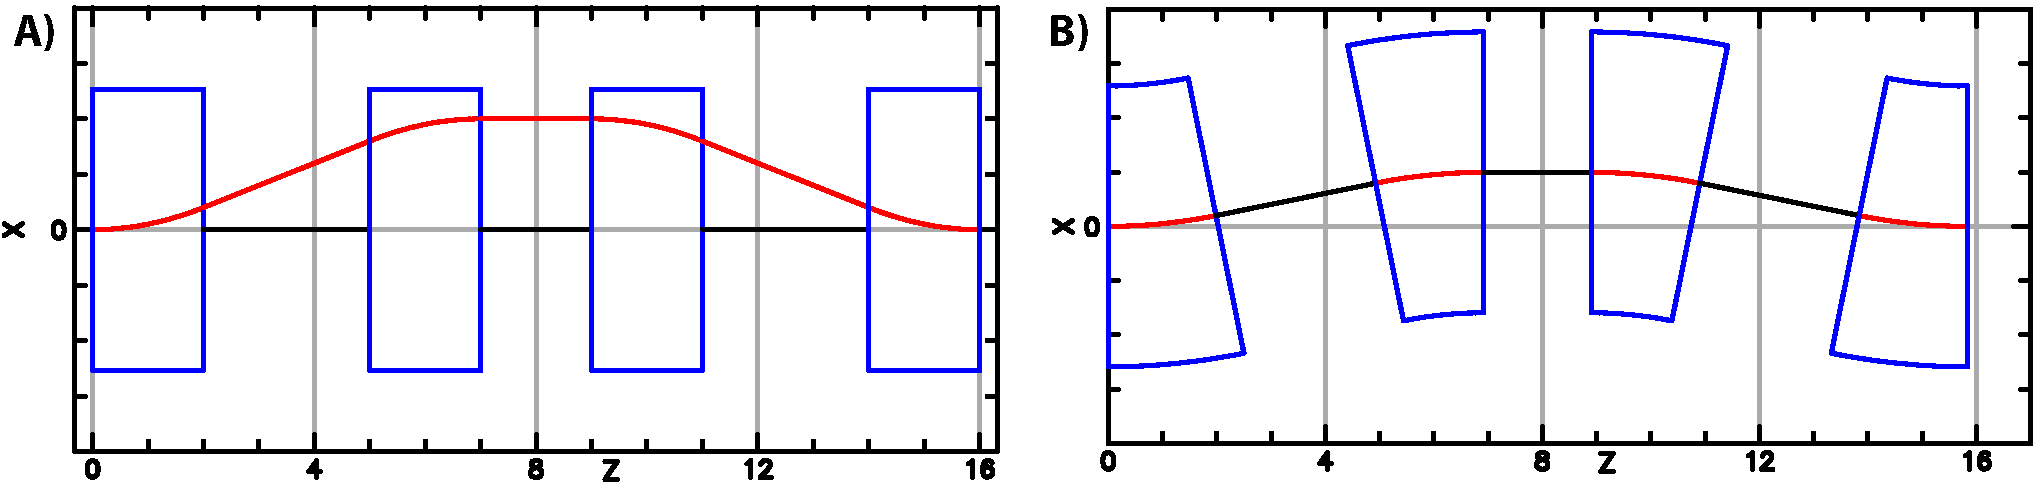
\includegraphics[width=5in]{chicane.pdf}
  \caption[Four bend chicane.]{Four bend chicane. A) Correctly implemented chicane. The red line is 
the beam orbit magnified by a factor of 100. B) Incorrectly implemented chicane where the \vn{g}
parameter of the bends is used to control the chicane strength instead of \vn{dg}.
  }
  \label{f:chicane}
\end{figure}

A \vn{chicane} is a series of bending magnets that shifts the beam trajectory in the transverse
plane while keeping the starting and ending trajectories constant. Chicanes are useful for doing
things like bunch compression or as a variable bunch time delay. An example four bend chicane is
illustrated in \fig{f:chicane}A. The lattice file for this is:
\begin{code}
  parameter[geometry] = open
  beginning[beta_a] = 20
  beginning[beta_b] = 20
  parameter[p0c] = 1e7

  bnd1: rbend, l = 2
  bnd2: rbend, l = 2
  d1: drift, l = 3
  d2: drift, l = 2

  chicane: overlay = {bnd1[dg]:-ge, bnd2[dg]:ge}, var = {ge}, ge = 2e-3

  c_line: line = (bnd1, d1, bnd2, d2, bnd2, d1, bnd1)
  use, c_line
\end{code}
The chicane is controlled by an overlay (\sref{s:overlay}) called \vn{chicane}. This overlay controls
the \vn{dg} attribute of the bends (alternatively the \vn{hkick} or \vn{b0} attributes could have
been used).

It is important to note that using \vn{g} instead of \vn{dg} to control the chicane strength
would be a mistake. [Or, alternatively, \vn{b_field} instead of \vn{db_field} if controlling the
unnormalized field.] This is illustrated in \fig{f:chicane}B where the chicane overlay was replaced
by:
\begin{code}
  chicane: overlay = {bnd1[g]:-ge, bnd2[g]:ge}, var = {ge}, ge = 1e-1
\end{code}
The problem here is that \vn{g} sets the reference orbit so varying \vn{g} will vary the physical
layout of the machine which is not what is wanted. Since the actual normalized field is \vn{g +
dg}, it is \vn{dg} that should be varied. Notice that in the case where \vn{g} is varied, the
bends are no longer rectangular. This is true since \vn{rbend} elements, when read in from the
lattice file, are converted to \vn{sbend} elements. In this case the converted bends have \vn{e1}
and \vn{e2} face angles of zero. When the \vn{chicane} overlay varies \vn{g}, the face angle remain
zero. That is, the bends will always be pure sector bends. [In a situation where, indeed, \vn{g} is
to be varied and it is desired to keep bends rectangular, the appropriate variation of the \vn{e1}
and \vn{e2} can be put in the controlling overlay.]

%------------------------------------------------------------------------------
%------------------------------------------------------------------------------
\Section{Programming With Bmad}
\label{s:bmad.program}

%------------------------------------------------------------------------------
\subsection{Modifying the Lattice Reference Energy}

Imagine the situation where you want to make a table of some property of the lattice as a function
of the reference energy of the lattice. 

Example: Looking at the spin resonance as a funtion of the reference energy

\begin{code}
program test

use bmad

implicit none

type (lat_struct), target :: lat
type (ele_struct), pointer :: ele0
type (coord_struct), allocatable :: co(:)
real(rp) e_tot, a_gamma, spin0(3)
integer i, ie_arc

!

ie_arc = 1850   ! Arc element
bmad_com%auto_bookkeeper = .false.
bmad_com%radiation_damping_on = .true.
bmad_com%spin_tracking_on = .true.

spin0 = [0.0_rp, 1.0_rp, 0.0_rp]
call bmad_parser ('lat.bmad', lat)
ele0 => lat%ele(0)

do i = -40, 0
  a_gamma = 40.0_rp + i /1d3
  e_tot = a_gamma * mass_of(electron$) / anomalous_moment_of(electron$)
  ele0%value(E_tot$) = E_tot
  call set_flags_for_changed_attribute (ele0, ele0%value(E_tot$))
  call lattice_bookkeeper(lat)
  call twiss_and_track(lat, co)
  print '(es12.4, f10.4, f10.3, 5x, 3f12.6)', E_tot, a_gamma, &
                          norm2(co(ie_arc)%spin - spin0), co(0)%vec(1)
enddo

end program
\end{code}

%------------------------------------------------------------------------------
\subsection{Changed Lattice Detection}

Suppose you have a program that takes lattice dependent quantities and, for say speed of execution
next time the program is run, saves these quantities to a file. Next time the program is run, you
want to know if the lattice has been modified between the time that the quantities were saved and
the present. If the lattice has been modified, the program will need to recalculate the
quantities. How can the program tell if there has been a modification?

The answer is that the \vn{lat_struct} has a parameter \vn{lat%creation_hash} which is computed
based on the modifiction dates of all the lattice files used to construct the lattice. Thus if this
hash value is saved with the lattice dependent quantities, the saved value can be compared to the
current value and if the values are different, a lattice file has been modified. 

Note: This test is a bit too stringent since if lattice files are moved 



%------------------------------------------------------------------------------
%------------------------------------------------------------------------------
\Section{Programming With PTC}
\label{s:ptc.program}


%------------------------------------------------------------------------------
%------------------------------------------------------------------------------
\Section{Programming With Tao}
\label{s:tao.program}


%------------------------------------------------------------------------------
%------------------------------------------------------------------------------
\Section{X-Ray Crystal Rocking Curve}






\end{document}







At some point you may want to do something beyond the capabilities of \tao and other \bmad based
programs. For example, 
In this case you have the option of writing a new \bmad based program from the ground up
or you can modify an existing program. 

Two sources of information for creating \bmad based programs
is the third section of the \bmad manual and the \bmad web site. In particular see the page:
\begin{display}
  \url{https://wiki.classe.cornell.edu/ACC/ACL/BuildSystem}
\end{display}
If you are interested in modifying \tao, further documentation can be found in the last section of 
the \tao manual.


At some point you might want to extend the capabilities of \tao. For example, to enable \tao to read
in data that you have collected from an experiment or to interface \tao to the control system for
your machine. 

create your own simulation program based upon the \bmad library. This is a large subject and this
section will just serve as a quick introduction on how to initially set things up. 

Also if you want to create 

Must use bash.
